\documentclass{article}
\usepackage[utf8]{inputenc}
\usepackage[italian]{babel}
\usepackage[T1]{fontenc}
\renewcommand{\baselinestretch}{1.5}

\title{EFM}
\author{matildetozzi}
\date{December 2020}

\usepackage{blindtext} %\blindtext

\usepackage{graphicx}
\graphicspath{ {./EFM_images/} }
\usepackage{wrapfig}
\usepackage{amsmath}
\usepackage{amssymb}
\usepackage{geometry}
 \geometry{
 a4paper,
 total={170mm,257mm},
 left=10mm,
 right=10mm,
 top=5mm,
 bottom=5mm,
}

\begin{document}
\thispagestyle{empty}
\textbf{Sistemi lineari di ODE} \quad
\textit{Soluzione}: $u(t)=Pe^{Bt}c \quad c:=P^{-1}C \quad B=P^{-1}AP$ \quad i) calcolo gli autovalori di A: $det(A-\lambda I)=0$ \quad ii) calcolo gli autovettori associati: $(A-\lambda I)\,v = 0$ ed eventualmente gli autovettori generalizzati $(A-\lambda_1 I)\, w_1 = v_1$ \quad iii) calcolo matrici P, B, $e^{Bt}$: $P=(v_n | w_m) \quad e^{Bt}=e^{Jt}=e^{\lambda t}\sum_{k=0}^{n-1}\frac{t^k}{k!}N^k$ 
|\textit{Punti di equilibrio}: $\frac{du}{dt}=0$ per capire se è stabile o instabile, fare grafico ($u,\frac{du}{dt}$) 
| \textit{Stabilità p.ti eq.}: verificare se una funzione V associata $\Bar{x}$ è di Lyapunov, i) $V \in C^1 (Q)$ ii) $V(\Bar{x})=0$ iii) $V(x)>0 \quad \forall x \in Q \backslash \{ \Bar{x} \}$ iv) $\frac{d}{dt}V(x(t))\leq 0 \Leftrightarrow \nabla V(x) \cdot f(x) \leq 0 \quad \forall x \in Q$
\begin{wraptable} {l}{8.6cm}
\begin{tabular}{c|c}
$\lambda$ di A & $\Bar{x}=0$ \\
\hline
\textit{tutti} p. reale <0 & glob.esp.asint.stabile \\ 
\textit{uno} p. reale >0 & instabile \\
\textit{tutti} p.real$\leq0$ e =0 semplici & stabile
\end{tabular}
\end{wraptable}
se è di Lyapunov \textit{in senso stretto}, c'è < in iv) e $\Bar{x}$ è asint. stab.
| \textit{Stabilità dell'eq.}: i) se A non singolare ($det(A)\neq 0$), solo $\Bar{x}=0$ ii) se A singolare, ker(A) ($\{ v\,|\, Av=0\}$) è uno sp. vett. di p. di eq. con $1\leq dim \leq n$ VD TABELLA
| \textit{Linearizzazione}: si trova in prima appross. $\frac{d}{dt}\eta (t) = f'(\Bar{u})\eta (t)$ i) f'<0 $\rightarrow$ asint.stabile ii) f'>0 $\rightarrow$ inst iii) f'=0 $\rightarrow$ sviluppare al II ord.
| \textit{Ritratto di fase (isocline)} 

\textbf{Sistemi di PDE} \quad 
\underline{Equazione del trasporto} $ \left\{ \begin{array}{l}
\partial_t u + v(x,t,u)\partial_x u = f(x,t,u) 
\\ u(x,0) = u_0 (x)
\\ (x,t) \in \mathbb{R} \times (0,\infty) 
\end{array}\right.$ $\rightarrow$
$ \left\{ \begin{array}{ll}
\frac{d}{dt}x(t) = v(x(t),t,\hat{u}(t)) & t \in (0,\infty) 
\\ \frac{d}{dt}\hat{u}(t)=f(x(t),t,\hat{u}(t)) &
\\ x(0)=x_0 \in \mathbb{R}, & \hat{u}(0)=u_0 (x_0)
\end{array}\right.$

\underline{Leggi di conservazione} $\partial_t u + F'(u)\partial_x u = 0,\, u=u(x,t), \, (x,t) \in \mathbb{R} \times (0, \infty)$ | \textit{caratteristiche} $x(t)=x_0 + F'(u_0 (x_0 ))t$ | \textit{t. prima intersezione} $t^* = -\frac{1}{F''(u_0 (x_m))u'_0(x_m)}$ con $x_m=\text{argmin}_{x_0 \in \mathbb{R}}(F''(u_0 (x_m))u'_0(x_m)) $
\underline{P. di Riemann} \textit{onda d'urto} s(t) cond. di Rankine-Hugoniot $\frac{d}{dt}s = \frac{F(u(s^+,t))-F(u(s^-,t))}{u(s^+,t)-u(s^-,t)}$ con $s(0)=p$
| \textit{onda di rarefazione} $u(x,t)=(F')^{-1}(\frac{x-x_0}{t-t_0})$ $(x_0,t_0)=(p,0)$
\begin{wrapfigure}{l}{10.7cm}
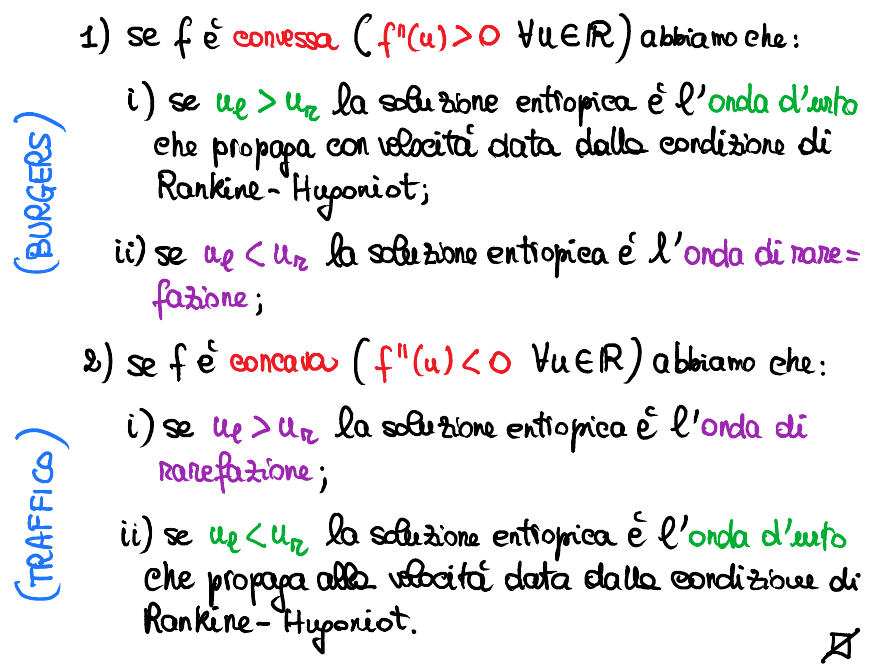
\includegraphics[width=5cm]{Sol_entropica.png}
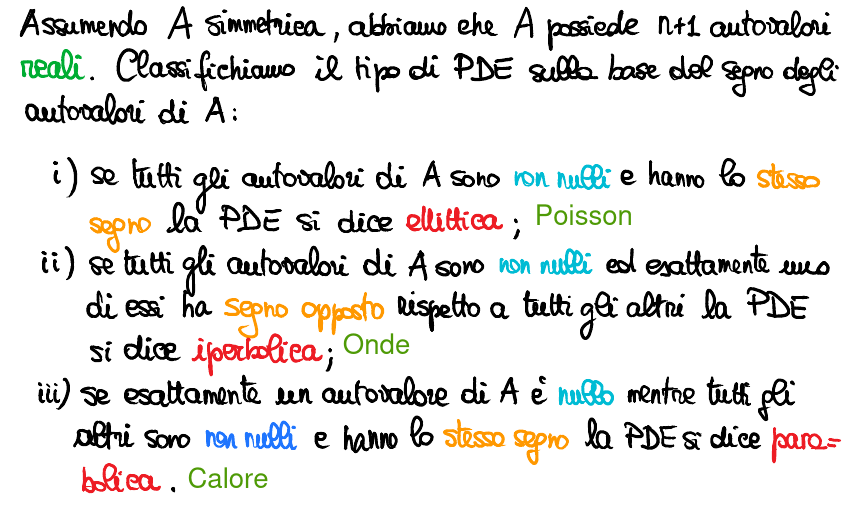
\includegraphics[width=6cm]{secondo_ordine.png}
\end{wrapfigure}
\underline{Equazioni del secondo ordine} A matrice coeff. $\partial^2_{y_i y_j}$
\underline{Equazione delle onde} $\partial_t^2u-c^2\partial_x^2u=f(x,t)$, $(x,t) \in \mathbb{R} \times (0,\infty)$, $u(x,0)=u_0(x)$, $\partial_tu(x,0)=u_1(x)$ 
$\rightarrow$
 $u(x,t)=\frac{1}{2}(u_0(x-ct)+u_0(x+ct))+\frac{1}{2c}\int_{x-ct}^{x+ct}u_1(z)\,dz+\frac{1}{2c}\int_0^t\int_{x-c(t-s)}^{x+c(t-s)}f(z,s)\,dz\,ds$ (senza f è la \textit{formula di D'Alembert}) $\bullet$ se \textit{cond. di Dirichlet} ($u(0,t)=g(t),\,t\in[0,+\infty)$), usi D'Alembert 
 in $x\geq ct$ e $g(t-\frac{x}{c})+\frac{1}{2}(u_0(x+ct)-u_0(ct-x))+\frac{1}{2c}\int_{ct-x}^{x+ct}u_1(z)\,dz$ in $0<x<ct$
 $\bullet$ se \textit{cond. di Neumann} ($\partial_xu(0,t)=h(t),\,t\in[0,\infty)$), usi D'Alembert in $x\geq ct$ e $\frac{1}{2}(u_0(ct-x)+u_0(x+ct))+\frac{1}{2c}(\int_0^{ct-x}u_1(z)\,dz + \int_0^{x+ct}u_1(z)\,dz)-c\int_0^{t-\frac{x}{c}}h(s)\,ds$ in $0<x<ct $
\underline{Soluzione per serie} $u(x,t)=\sum_{k=0}^\infty \hat{u}_k(t)\psi_k(x)$ 
\quad $\hat{u}_k(t)=\hat{u}_{0,k}\cos (c\sqrt{\lambda_k}t)+\frac{\hat{u}_{1,k}}{c\sqrt{\lambda_k}}\sin (c\sqrt{\lambda_k}t)$
\quad $\hat{u}_{0,k}$ t.c. $\sum_{k=0}^\infty \hat{u}_{0,k}\psi_k(x)=u_0(x)$
\quad $\hat{u}_{1,k}$ t.c. $\sum_{k=0}^\infty \hat{u}_{1,k}\psi_k(x)=u_1(x)$
\quad $\psi_k(x)=\Tilde{C}_{1,k}\cos (\sqrt{\lambda_k}x)+\Tilde{C}_{2,k}\sin (\sqrt{\lambda_k}x)$
\quad i) $\Tilde{C}_{1,k}$, $\Tilde{C}_{2,k}$ e $\lambda_k$ calcolati applicando cond. Neumann/Dirichlet a $\psi_k$ 
ii) trovare $\hat{u}_{0,k}$ e $\hat{u}_{1,k}$ iii) mettere insieme
\quad se problema in 2D, come prima ma $u(x,y,t)=\sum_{k=0}^\infty \hat{u}_{k,j}(t)\psi_k(x)\varphi_j(y)$, coppia autovalore-autofunzione ($\psi_k(x),\mu_k$), ($\varphi_j(y),\varepsilon_j$) e $\lambda_{k,j}=\mu_k+\varepsilon_j$
\underline{Equazione del calore}
$\partial_tu-D\,\partial_x^2u=0$ in $\mathbb{R}\times (0,+\infty)$ , $u = \delta(x)$ in $\mathbb{R}\times \{ 0 \}$ e $u \rightarrow 0$ per $|x| \rightarrow \infty \, \forall t>0$
\textit{Soluzione fondamentale} distribuzione gaussiana $u(x,t)=\frac{1}{\sqrt{4 \pi Dt}}\exp{(-\frac{x^2}{4Dt})}$ con media = 0 $\forall t>0$ e varianza = $2Dt$
\underline{Formula di rappr della sol di un generico problema di Cauchy}
$\left\{ \begin{array}{rl}
\partial_tu-D\,\Delta u=0 & \mathbb{R}^n \times (0,+\infty) \\
u=u_0 & \mathbb{R}^n \times \{ 0 \} \\
u \rightarrow 0 & |x|\rightarrow \infty
\end{array}\right.$ $\rightarrow$
$u(x,t) = [(\frac{1}{(4\pi Dt)^{n/2}}\exp{(-\frac{|x|^2}{4Dt})})\ast u_0](x,t) = \int_{\mathbb{R}^n}\frac{1}{(4\pi Dt)^{n/2}}\exp{(-\frac{|x-y|^2}{4Dt})}u_0(y)\,dy $
\underline{Equazione del calore su un dom spaz limitato}

$\left\{ \begin{array}{rll}
\partial_tu-D\, \Delta u =0 & \Omega \times (0,+\infty) & \text{\underline{Soluzione per serie} simile a sopra, ma $u(x,t)=\sum_{k=0}^{+\infty}\hat{u}_{0,k}\exp(-k^2\pi^2Dt)\cos(k\pi x)$}\\
u=u_0 & \Omega \times \{0\} & \text{se $u_0 = \delta(x)$, usare \underline{Ansatz} $u(x,t)=v(x,t)w(t)$}\\
-D\,\nabla u\cdot\underline{n}=0 & \partial\Omega\times(0,+\infty) & \text{\underline{energia} = integrale quantità al quadrato, fare $\frac{d}{dt}\int_\Omega |\bullet|^2 \,dx$ e usare Grönwall}
\end{array} \right.$



W DI LAMBERT $W(z)$ inversa di $ze^z$
T. DIVERGENZA $\int_\Omega \text{div}(u)\,dx = \int_{\partial \Omega} u \cdot n\,d \sigma$
T. DIVERGENZA+LAPLACIANO $\int_\Omega u \Delta u\,dx = \int_\Omega \text{div}(u \nabla u)\,dx - \int_\Omega |\nabla u |^2 \,dx = \int_{\partial \Omega} u \nabla u \cdot n\,d \sigma - \int_\Omega |\nabla u |^2 \,dx$
DERIVATA DI $u_-$: $\partial_t (u_-)^2 = -2u_- \partial_t u$
GRÖNWALL \underline{differenziale} $\frac{d}{dt}u(t)\leq B(t)u(t) \Rightarrow u(t)\leq u_0 \exp(\int_{t_0}^tB(s)\,ds)$
\underline{integrale}
$u(t)\leq A(t)+\int_{t_0}^tB(s)u(s)\,ds \Rightarrow u(t)\leq A(t)+\int_{t_0}^tA(s)B(s)\exp(\int_s^tB(z)\,dz)\,ds$
DISUGUAGLIANZA DI POINCARÉ (-WIRTINGER) $\int_\Omega |u\boldsymbol{(}-\langle u \rangle\boldsymbol{)}|^2\,dx \leq C \int_\Omega|\nabla u|^2\,dx$
METODO DEL FATTORE INTEGRANTE 
$y'-ay=b$ $\rightarrow$
$\mu(t)=\exp(-\int a(t)\,dt)$ $\rightarrow$
$\mu(t)(y'-ay)=\mu(t)b$

\end{document}
    